\documentclass[a4paper, 12pt, onecolumn]{article} 

% To change the distance between the columns when using `twocolumn`:
\setlength{\columnsep}{0.5in} % Source: tex.stackexchange.com/a/24563/110560


%% Read https://texblog.org/2012/08/29/changing-the-font-size-in-latex/ for reference on font sizes.

% For margins. 
% Source: kb.mit.edu/confluence/pages/viewpage.action?pageId=3907057. 
% Also see: https://www.sharelatex.com/learn/Page_size_and_margins
\usepackage[margin=1.0in]{geometry}  

 % For the "comment" environment to make LaTeX comments
\usepackage{verbatim} 

% For equations \begin{equation*}:
\usepackage{amsmath, amssymb}  

% For tables using \begin{longtabu}:
\usepackage{tabu, ltxtable, tabularx, longtable}

% For captions on longtabu, see tex.stackexchange.com/q/268927/110560
\usepackage{caption}
\captionsetup[longtable]{skip=9pt, margin=0.1\textwidth,
	 justification=justified, singlelinecheck=false}	% Source: tex.stackexchange.com/a/95208/110560 and tex.stackexchange.com/a/3178/110560 and tex.stackexchange.com/a/88817/110560 and tex.stackexchange.com/a/37793/110560

% For images using \begin{figure} and for \scalebox{}:
\usepackage{graphicx}
\graphicspath{Images/}  % Location of the graphics files (set up for graphics to be in PDF format)

% For using bullets in description lists.
\usepackage{enumitem}

% For Neural Network Diagrams, see http://tex.stackexchange.com/a/132471/110560
\usepackage{tikz}
\usetikzlibrary{matrix,chains,positioning,decorations.pathreplacing,arrows}


\addtolength{\footnotesep}{1mm} % Source: tex.stackexchange.com/a/141938/110560.

% For URLs with \url{blahblahblah}
\usepackage{url} % Source: http://tex.stackexchange.com/a/40222/110560

% For rotating figures with \begin{sidewaysfigure}
\usepackage{rotating}


% For code, using as \begin{lstlisting}. Source: http://stackoverflow.com/a/3175141/4900327
\usepackage{listings}	

% For side-by-side figures, see: tex.stackexchange.com/a/37582/110560
\usepackage{subfigure}



% Source: http://stackoverflow.com/a/3175141/4900327
\lstset{frame=tb,
	language=bash,
	aboveskip=3mm,
	belowskip=3mm,
	showstringspaces=false,
	columns=flexible,
	basicstyle={\small\ttfamily},
	numbers=none,
	numberstyle=\tiny\color{gray},
	keywordstyle=\color{blue},
	commentstyle=\color{gray},
	stringstyle=\color{olive},
	breaklines=true,
	breakatwhitespace=true,
	tabsize=3
}

% For quotations. Source: 
\usepackage[utf8]{inputenc}
\usepackage{csquotes}

\begin{document}
	
	

%\hspace{5em} Normalization:
%\begin{equation*}
%x_{i, 0...1} = 
%\frac	{ x_{i} - x_{min}	}
%{ x_{max} - x_{min}	}
%\end{equation*}

	
%% NSL Test Set with SMOTE and Random Undersampling:
%\centering \begin{longtabu} to \textwidth {| l | c | c | c | c | } \hline
%	& Precision & Recall	& F1 score  & Support	\\ \hline
%	DoS   	& 93\%   	& 84\%      & 88\%      & 7457		\\ \hline
%	Normal	& 73\%   	& 95\%      & 83\%      & 9710		\\ \hline
%	Probe 	& 64\%   	& 57\%      & 60\%      & 2421		\\ \hline
%	R2L   	& 64\%   	& 12\%      & 20\%      & 2754		\\ \hline
%	U2R 	&  5\%     	& 16\%      & 8\%       & 200		\\ \hline
%	Total 	&  76\%     & 76\%   	& 76\%   	& 22542		\\ \hline
%	\caption{Decision Tree on NSL Test Set with SMOTE and Random Undersampling. Total Accuracy = 76.32\%}
%\end{longtabu}


%\begin{figure}[!h]
%	\centerline{}
%	\caption{An Artificial Neural Network with one hidden layer, working on a dataset with three predictors and two target classes.}
%	\label{fig: ANN}
%\end{figure}


%\input{"Sections/Notation and nomenclature"}
%\input{"Sections/The goal of Backpropagation"}
%\input{"Sections/Forward pass"}


%\scalebox{1.7}{
	%{}^{14}\text{C}^{15}	%% Source: tex.stackexchange.com/a/30563/110560
	
%}

%\input{"Diagrams/Generic Neuron"}
%\\
%\centering Generic Neuron
%\input{"Diagrams/Example Network"}


\title{Mobile-controlled wireless rover with IR sensors}

\author{
	Abhishek Divekar (131080051) \\ 
	Vaibahav Savla (131080051) \\ 
	Meet Parekh (131080051) \\ 
	\\
	Veermata Jijabai Technological Institute\\
	H. R. Mahajani Marg, Matunga, Mumbai - 400031,\\ 
	Maharashtra, India\\
}

\date{}	%Source: tex.stackexchange.com/a/2761/110560

\maketitle

\thispagestyle{empty}

\begin{abstract}
	Wireless, sensor-driven robotics is a discipline with ready applications in military, factory and civilian uses. While they initially lacked robustness due to the inherent problems associated with wireless technology such as fluctuating signal strength and difficulty in debugging, the technology has now matured such that several critical services and mechanisms now operate wirelessly. Coupled with the ubiquity of Wireless LAN technology and the Internet, we find that there are some interesting use cases for remotely-controllable vehicles. 
	
	In this paper we both provide the specifications for and build a movable robot which may be controlled from any device connected to the same Wireless LAN, via a Web 2.0 interface. IR sensors feed information back to the controlling human, allowing them to maneuver accordingly based on the terrian.
	
	While not suitable for industry or military grade applications, this setup was found to be robust from an experimental and academic viewpoint.
\end{abstract}



\section{Introduction}

\begin{description}[font=\quad $\circ$, topsep=-2pt, itemsep=2pt]
	\item Rovers have been widely employed by military and research community (space research) to explore unknown terrains. However rovers have also been in use for simpler applications such as monitoring of different zones on the factory floor. Be it simple or complex rover, they present two major challenges:
	
	\begin{enumerate}[itemsep=0em]
		\item Interaction with the environment
		\item Wireless control
	\end{enumerate}
	
	\item In comparison with the scientific Mars rovers which are voluminous beasts of the order of a few hundred kilograms \cite{RobotSizes}, our rover is a simple three-wheeled bot weighing slightly more than a 1500 grams. The motors power the back wheels and the front wheel is simply a ball-bearing with a low coefficient of friction, allowing the rover to move quickly over smooth surfaces.

	\clearpage
	\quad A block-diagram of the overall hardware system is as follows:

	\begin{figure}[ht]	% Source: http://tex.stackexchange.com/q/131259/110560
		\centering
		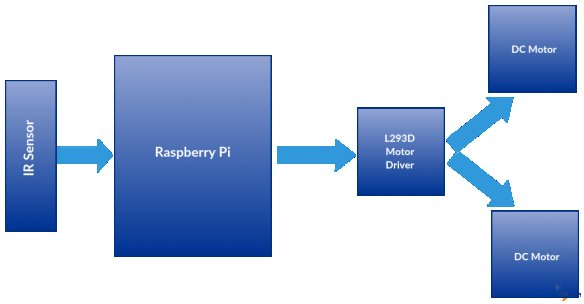
\includegraphics[width=\linewidth]{"./system_diagram.jpg"}
		\caption{System diagram of the rover}
		\label{fig:System Diagram}
	\end{figure}

	\item The microcontroller used is the Raspberry Pi 3, a popular and well-supported hobbyist board. It comes bundled with an onboard Wireless chip and 40 General Purpose Input/Output pins for interfacing with the motors and IR sensors. Power is supplied via a pair of 9v batteries (to the motors) and a 5600 mAh powerbank (to the Pi). The controlling GUI is served by a Python Django server running on Raspbian, a Linux-based distribution installed on the Raspberry Pi’s external memory.

	\item The DC motors that move the rover around are standard 300 rpm high-torque motors \cite{300RPMMotors} (low torque motors were unsuccessful in moving the rover on even flat surfaces). The power is delivered via 9v batteries, and controlled via a L293D motor driver. 


	\item An important module of the rover is the trio of IR sensors on the bottom panel, around one inch above the ground. They are used to detect the terrain (black or white) and can be used for line-following even in dim environment. While sufficient for our current purposes, it is possible to replace them with complex, application-specific sensors if required e.g. landmine-detection apparatus for military use cases. \\

	\begin{figure}[ht]	% Source: http://tex.stackexchange.com/q/131259/110560
		\centering
		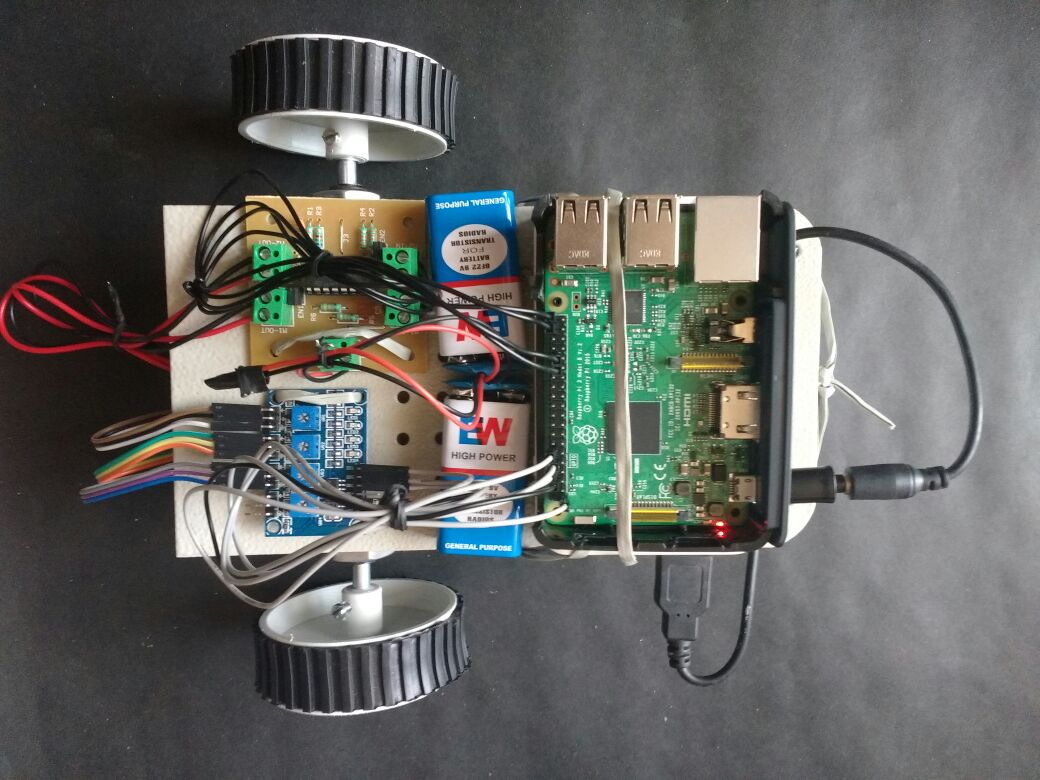
\includegraphics[width=\linewidth]{"./bot-pic-top.jpg"}
		\caption{A photograph of the assembled rover}
		\label{fig:BotPicTop}
	\end{figure}
	
\end{description}

While not nearly state-of-the-art, this setup is sufficient for the proof-of-concept which we build.



\clearpage


\section{Motivation}


\quad \quad The main aim of the project is to learn about embedded systems as a whole, and along the way display the applicability and robustness of wireless technology in robotics. We do so using a movable, proof-of-concept rover which we then control using a GUI interface accessible through either a mobile phone or laptop, anywhere in the vicinity. A simple extension of this notion would allow the control of robots in other countries or even on other planets. 


\section{Problem Definition}

\begin{enumerate}
	\item To construct a movable robot, with a 15x8 chassis, two wheels and three IR sensors attached to a makeshift cardboard bottom, and a Raspberry Pi 3B and DSG powerbank secured to the top. The IR sensor board and motor drivers are secured to the chassis with electrical tape or plastic cords to prevent movement.
	
	\item The Raspberry Pi automatically connects to a known Wireless LAN at bootup, thus allowing unsupervised bootups at regular intervals.
	
	\item A Web 2.0 interface would be served via a Python Django server to a computer ${}^{\ref{WhatsAComputer}}$ connected to the same Wifi network as the Pi. This interface serves the controls \textit{"Forwards"}, \textit{"Backwards"}, \textit{"Left"}, \textit{"Right"} and \textit{"Stop"}. The interface is served at an IP address known to the computer, removing the problem of reconfiguration. 

	\footnotetext[1]{\label{WhatsAComputer} Note that our only criterion for \textit{computer} is a device with a JavaScript-enabled web browser that is able to communicate via HTTP requests. We may thus use mobile phones (Android, iOS etc.) or laptop or desktop computers to access this interface.}	% Source for footnotes: latex-tutorial.com/tutorials/beginners/07b-footnotes/
	
	\item The interface would additionally display the status of three IR sensors as binary values, e.g. $010$, indicating the middle senor was triggered. This would be updated every few seconds without reloading the page. This is for reference of the human controller, similar to a video feed (which was infeasible due to bandwidth constraints).
	
	\item On clicking one of the buttons, a request would be sent over the Wireless connection to the Django server, which would in turn send a message to the motor drivers, moving the rover in the desired direction (or stopping it). 

\end{enumerate}

Note that this is a proof-of-concept project. Every stage would require changes in hardware materials and electronics to build a workable rover system.



\clearpage

\section{Methodology and Implementation}
	
	\subsection{Hardware ${}^{\ref{HardwareSource}}$ }

	\begin{enumerate}[topsep=-2pt, itemsep=10mm]
		\item \textbf{Raspberry Pi 3 Model B:} 
		
			The Raspberry Pi 3 is a hobbyist microcontroller board which can be used for a variety of embedded systems projects. 
		
			It's specifications ${}^{\cite{RPi3BSpecs}}$ include:
			\begin{description}[font=\quad $\circ$, topsep=-2pt, itemsep=2pt]
				\item Broadcom BCM2837 64bit ARMv7 Quad Core Processor powered Single Board computer running at 1.2GHz
				\item 1 GB RAM
				\item BCM43143 WiFi on board
				\item 4 USB 2.0 ports
				\item 40 GPIO pins${}^{\ref{fig: Raspberry Pi 3B pin diagram}}$ (General Purpose Input Output)
				\item Full HDMI port
				\item Micro SD card slot (an 8Gb SanDisk MicroSD was used)
			\end{description}
			
			\begin{figure}[!h]
				\centering
				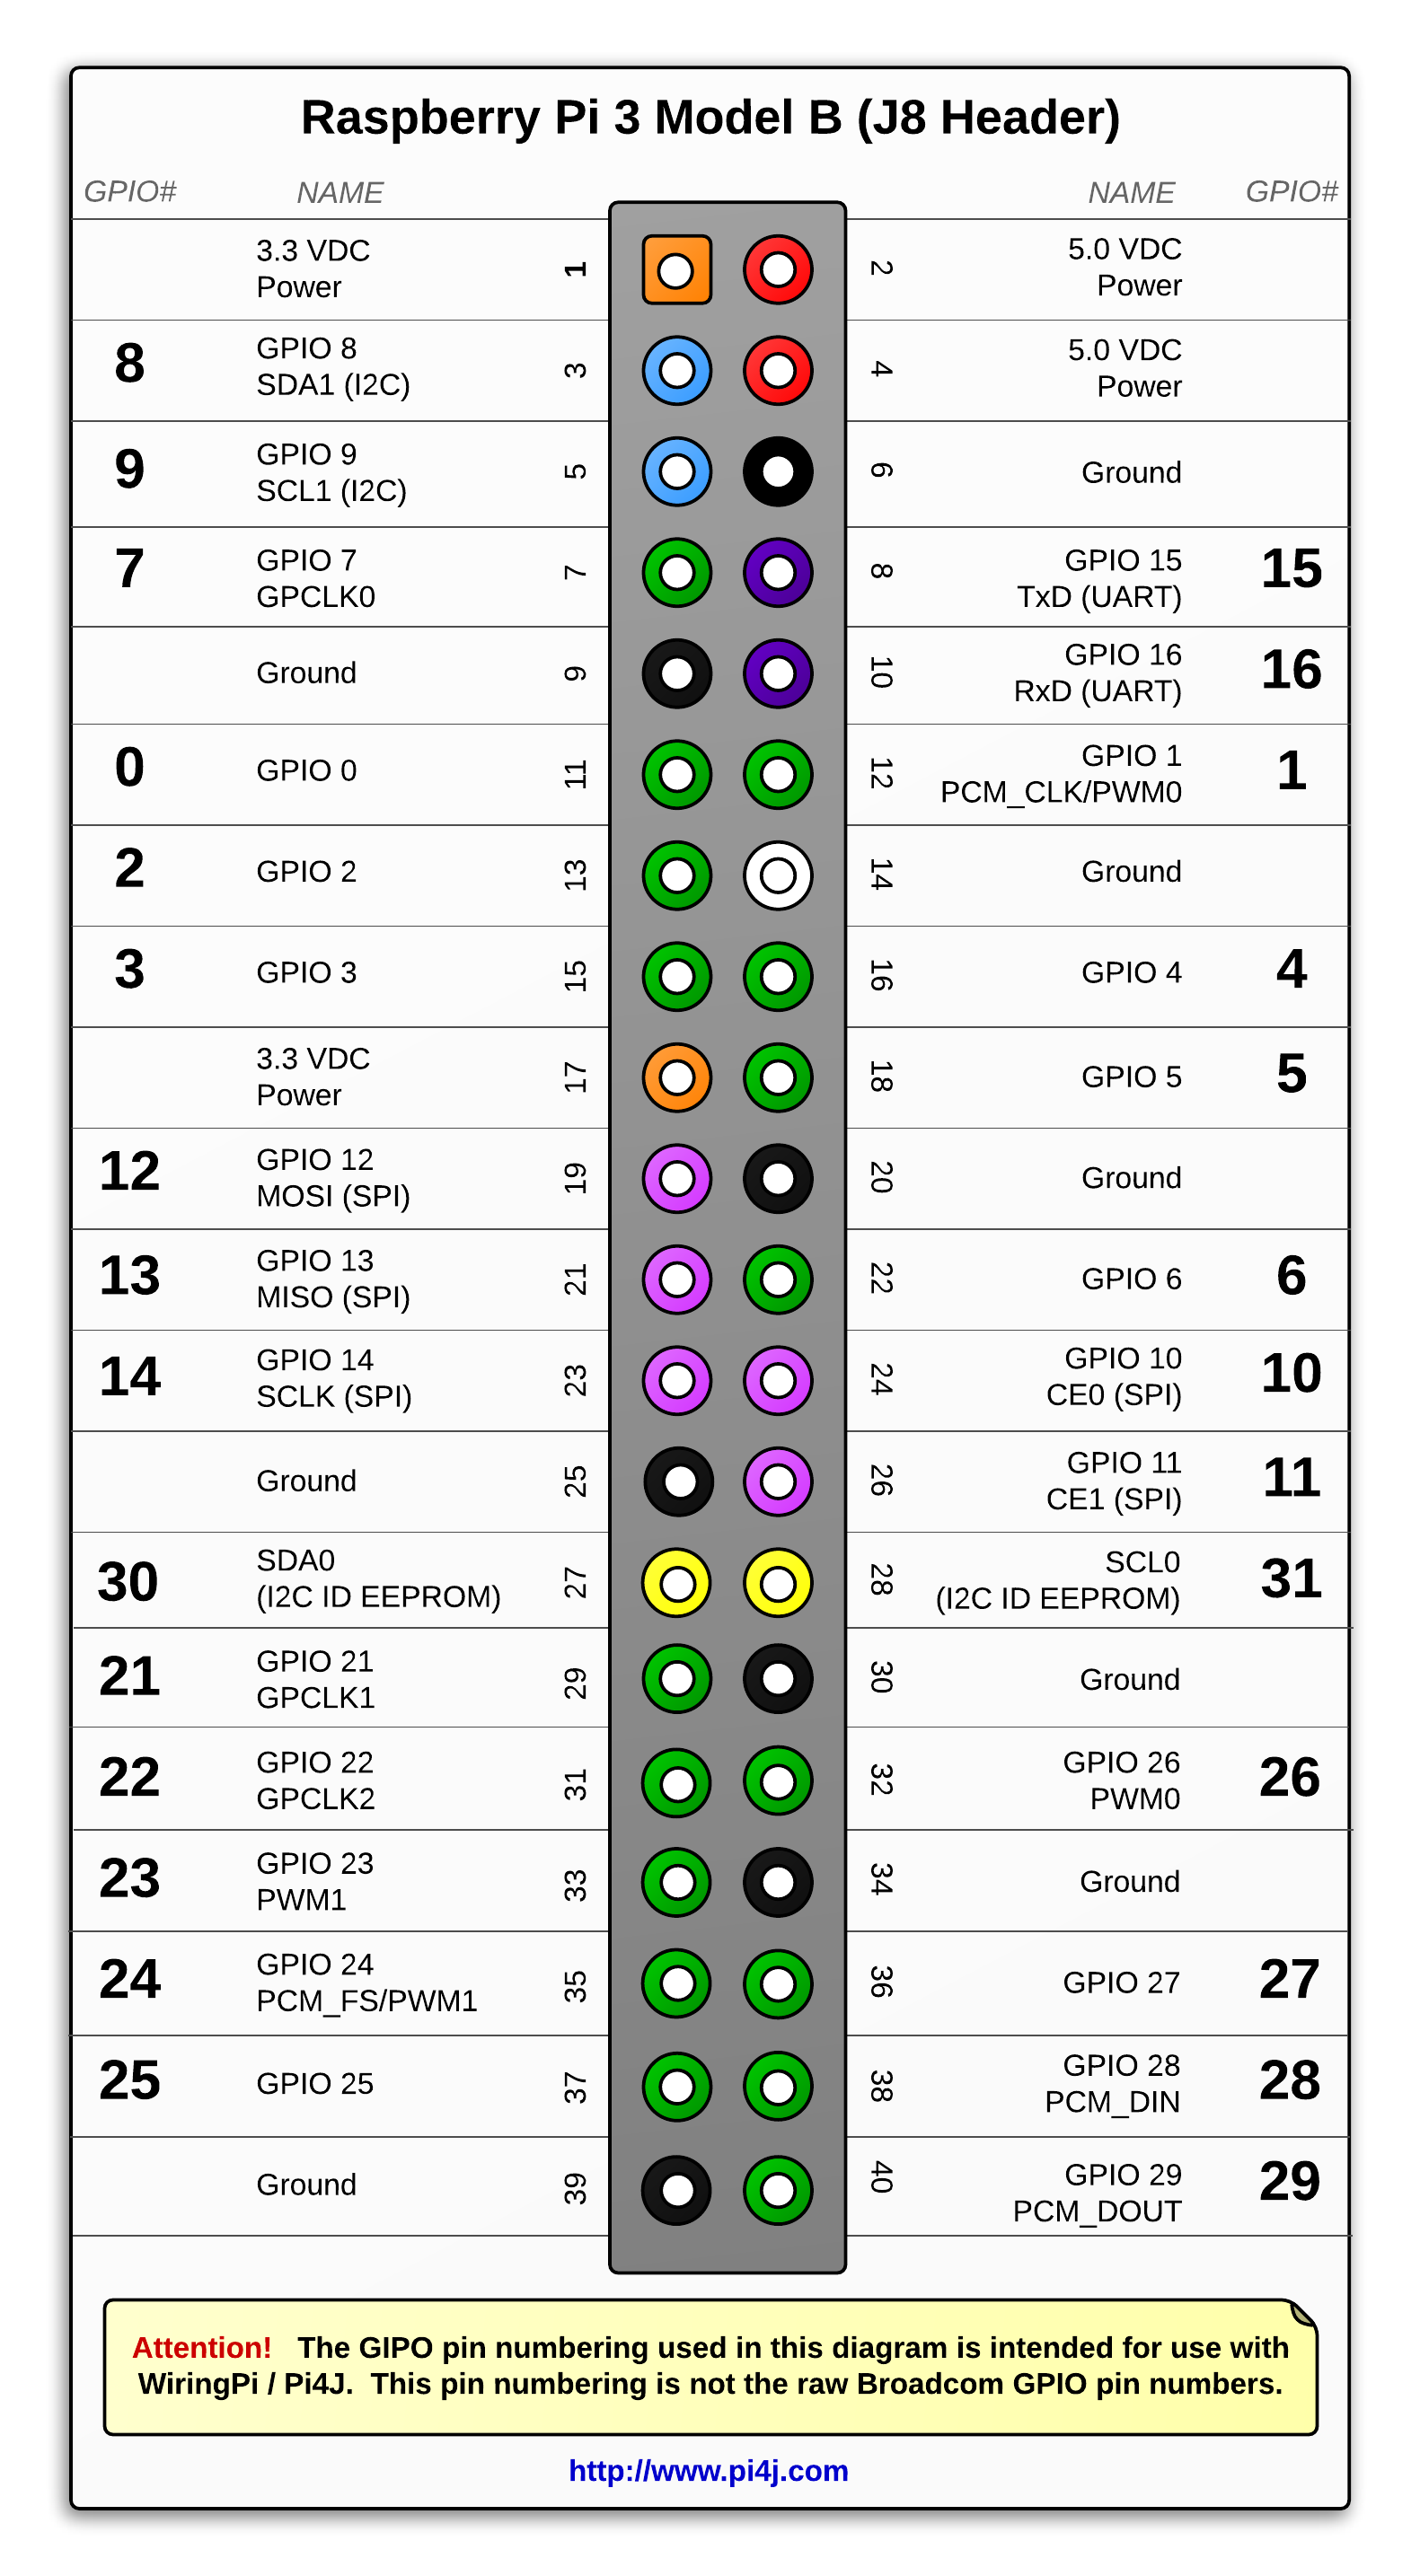
\includegraphics[width=0.42\linewidth]{"./raspberry-pi-3b-pin-diagram-j8header.png"}
				\caption{Raspberry Pi 3B pin diagram}
				\label{fig: Raspberry Pi 3B pin diagram}
			\end{figure}
			
			
			\footnotetext[1]{\label{HardwareSource} Most hardware for this project was obtained from specialty electronic stores around Mumbai. The Raspberry Pi 3B was borrowed from Prof. Bhole, Computers and Information Techonolgy Department, VJTI. We did our best not to alter his existing configurations.}
		
		
		
			
		\clearpage
		
		\item \textbf{Wheels and motors:} 
		
			The robot moves using two wheels each driven by a 300 RPM DC motor. These DC motors are connected with L293D IC which provides and H bridge to turn one motor and other off or both simultaneously in same direction or different direction. 
		
		
		\item \textbf{L293D Motor Driver:} 
		
			A quadruple high-current half-H driver. The L293D is designed to provide bidirectional drive currents of up to 600-mA at voltages from 4.5 V to 36 V. This allows the wheels to move in both directions and also turn left and right. ${}^{\cite{L293D_MotorDriver}}$
		
		
			We connect this driver${}^{\ref{fig: L293D Motor Driver pin diagram}}$ to the following pins of the Raspberry Pi:
	
			\tabulinesep=6pt	% Source: tex.stackexchange.com/a/207146/110560
			\begin{longtabu} to \textwidth {| c | c | } \hline
				\centering 
				Raspberry Pi 3B & L293D \\ \hline
				GPIO 29 (pin 40) & VCC \\ 
				GPIO 28 (pin 38) & GND \\ 
				GPIO 26 (pin 32) & GND \\ 
				Ground (pin 30) & GND \\ \hline
				\caption{Connections of Raspberry Pi to L293D Motor Driver}
			\end{longtabu}
			
			\begin{figure}[!h]
				\centering
				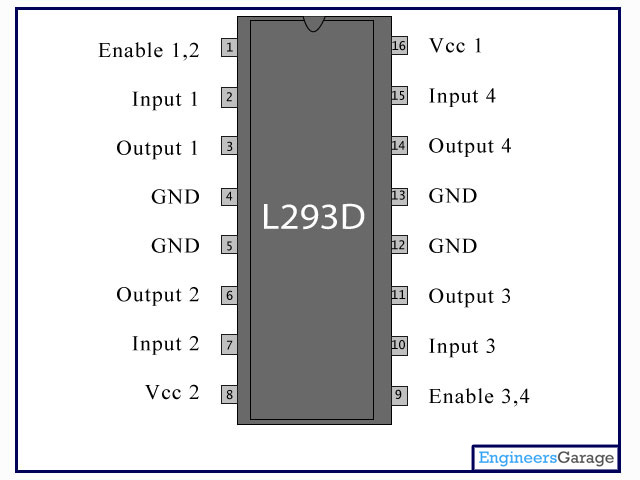
\includegraphics[width=0.5\linewidth]{"./L293D.jpg"}
				\caption{L293D Motor Driver pin diagram}
				\label{fig: L293D Motor Driver pin diagram}
			\end{figure}
			
			
			 \begin{figure}
				\centering
				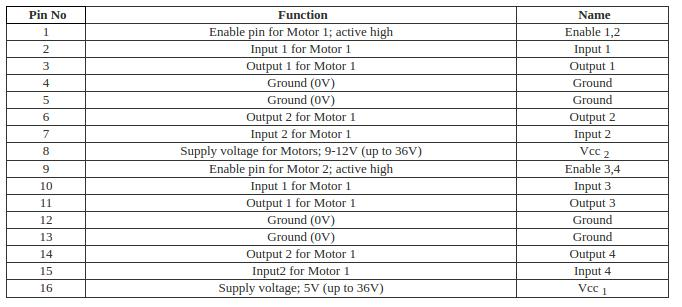
\includegraphics[width=0.9\linewidth]{L293D_pin_description}
				\caption{L293D pin description}
				\label{fig:L293D_pin_description}
			\end{figure}

			 
		 
		\item \textbf{IR sensors:} 
		
			In the rover, IR sensors are used to perform line-following on black or white striped lines. 
		
			IR sensors work on the principle of reflectance where there is one transmitter and one receiver. The transmitter transmits InfraRed rays which are received by the receiver to complete the circuit, due to which current flows through it. ${}^{\ref{fig:IR_transmitter_reciever}}$

			\begin{figure}
				\centering
				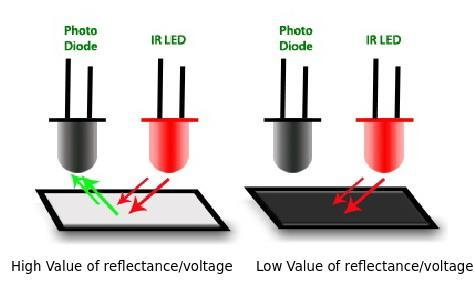
\includegraphics[width=0.6\linewidth]{IR_transmitter_reciever}
				\caption{The working of IR sensors}
				\label{fig:IR_transmitter_reciever}
			\end{figure}
			
			
			Dark colors are good absorber of rays, and they reflect very few of the IR rays falling on it. Due to this phenomenon, using a dark color as the background and white color as line allows to distinguish the path from the background as only white color will be detected by the sensors. 
			
			
			The sensitivity towards black and white of the IR sensor is adjusted by turning the potentiometer knobs on the top of each IR sensor.

	\end{enumerate}
	
	
	
	
	
	
	
	\subsection{Software}
	
	\begin{enumerate}[topsep=-2pt, itemsep=10mm]
		\item \textbf{Raspbian Jesse:} 
		
			It is a full-featured Linux operating system running a version of the Linux kernel and drivers, allowing seamless integration with external hardware such as cameras, ethernet, and Wireless LAN connections. Raspbian is highly optimized for the Raspberry Pi line's low-performance ARM CPUs.
			
			Raspbian uses PIXEL, Pi Improved Xwindows Environment, Lightweight as its main desktop environment as of the latest update. It is composed of a modified LXDE desktop environment and the Openbox stacking window manager with a new theme and few other changes.${}^{\cite{RaspbianPIXEL}}$ 
			
			The Raspbian operating system is based on Debian Linux, and the different versions of Debian are named after characters from the “Toy Story” films.${}^{\cite{RaspbianNaming}}$
		
		
		\item \textbf{Python:} 
		
		
		Python is an open-sourced, general-purpose programming language that is highly suited for writing short scripts without a log of boilerplate. First developed in 1995, it is one of the most popular programming languages that uses \textit{dynamic typing}. Python code files (.py) are compiled down to bytecode to run on the Python \textit{virtual machine}. 
		
		Python is a mainstay in Linux, and it is installed by default in almost all Linux distributions, including Raspbian. Despite it's simplicity, it is very powerful. 
		
		Because of the \textit{RPi} library, integrating Python into robotics experiments using the Raspberry Pi becomes particularly easy. We will often use \textit{RPi.GPIO} to send and receive inputs from the GOPI pins, controlling the motors. 
		
		
		\item \textbf{Django server:}
		
		Django is a high-level Python Web framework that encourages rapid development and clean, pragmatic design. ${}^{\cite{DjangoDescription}}$ It is often used to host large production websites. It is incredibly easy to install, as it is fully encapsulated into a Python library and thus installable with Python \textit{pip} via the command: 
		%Source: http://stackoverflow.com/a/3175170/4900327
		\begin{verbatim}  
			$ pip install django
		\end{verbatim}
		
		It is a testament to the Raspbian OS and the Django project that it is able to run the Django server as an extremely lightweight hosting server, which can be configured to receive requests from other computers on the same Wifi network by binding the runtime to receive requests from a static IP address. 
		
		We use Django to serve the frontend GUI interface on an HTTP GET request, and one clicking a button, we visit the appropriate link (e.g. \url{172.168.42.1/controls/left}) and perform the action specified there. The server imports the \textit{RPi.GPIO} package and sets the pins high or low, depending on the command. This in turn causes the 
		
		We also use the frontend to display the current status of the IR sensors as a string of zeros and ones, such as:
		
		\begin{equation}
			\begin{bmatrix}
			0 & 1 & 1
			\end{bmatrix}
		\end{equation}
		
		Which says the middle and right IR sensors are triggered, meaning that portion of the ground is white or light-colored. We retrieve this information using an AJAX call to \url{172.168.42.1/ir-sensors} and display it on the frontend. We update this value every 0.5 seconds using an AJAX call loop.
		
		
		\item \textbf{Bash:} 
		
		Bash scripts or shell scripts are command-line script files (.sh) which run on the Linux platform, allowing us to perform different OS-level functions using system calls. We specify different arguments and flags to change the behavior of the function called. The executable for these are stored in \url{/usr/bin}
		
		In our rover, we want the server to start automatically on boot, so we must create a shell script which gets the IP address that the raspberry pi is connected to and then runs the Django server from that address, as described in \cite{DjangoSameWifiCode}. This allows computers on the same wifi network as the Pi to connect to the Pi and send requests and receive responses from the Django server, which in turn allows us to control the rover's movement.
		
	\end{enumerate}
	
	

\clearpage

\section{Objectives}

\begin{enumerate}
	\item To make a rover with basic embedded systems architecture such as wheels, motors, chassis and battery.
	
	\item To program a Django server hosted on a Raspberry Pi 3 with the capability to wirelessly accept and respond to the requests \textit{"Forward", "Backward", "Left", "Right" and "Stop"} which can be sent by a human located remotely over a Wireless network.
	
	\item To provide feedback to the user from IR sensors positioned along the bottom of the rover, through a web-based interface accessible on any web-browser enabled device (Android, iOS, Windows, MacOSX and Linux).
	
	\item Learn about the challenges faced in the design and implementation of embedded systems as whole.
	
\end{enumerate}

\input{"Existing Systems"}

\clearpage 

\section{Implementation}

	Once we have connected the Raspberry Pi to the various hardware modules and ensured that the \textit{Raspbain Jesse} installation and \textit{Django server} are working, we may then proceed to create the following code files in a directory \texttt{es\_project} in the home directory of the Raspbian installation. 

%	\clearpage
%	\begin{figure}
%		\centering
%		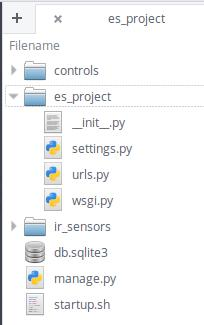
\includegraphics[width=0.3\linewidth]{es_project_directory_1}
%		\caption{}
%		\label{fig:es_project_directory_1}
%	\end{figure}
	
	\begin{figure}
		\hfill
		\subfigure[Main directory \texttt{es\_project/}] {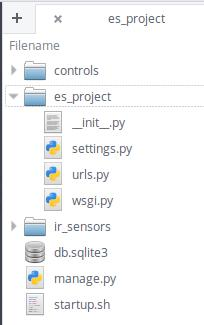
\includegraphics[height=6cm]{es_project_directory_1}}
		\hfill
		\subfigure[Sub directory  \texttt{controls/}]{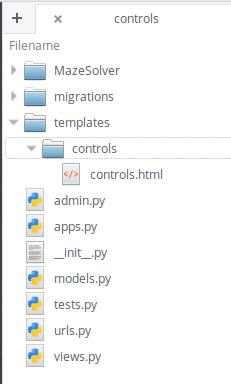
\includegraphics[height=5cm]{es_project_directory_2}}
		\hfill
		\subfigure[Sub directory  \texttt{ir\_sensors/}]{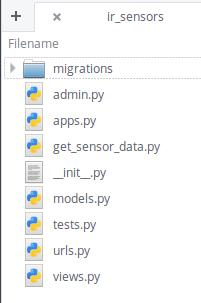
\includegraphics[height=5cm]{es_project_directory_3}}
		\hfill
		\subfigure[Sub directory  \texttt{MazeSolver/}]{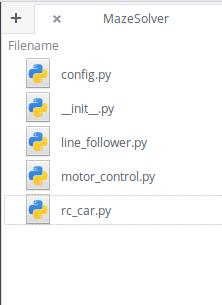
\includegraphics[height=5cm]{es_project_directory_4}}
		\hfill
		\caption{Django project directory layout}
	\end{figure}
	
%	\begin{figure}
%		\centering
%		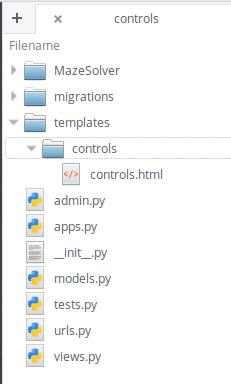
\includegraphics[width=0.3\linewidth]{es_project_directory_2}
%		\caption{}
%		\label{fig:es_project_directory_2}
%	\end{figure}

	
	As a reference, in general the steps outlines in the Django tutorial \cite{DjangoTutorial} should be followed, but some files were modified by us; those changes have been included below.
	
	\begin{description}[font=\quad $\circ$, topsep=6pt, itemsep=3em]
		\item \texttt{es\_project/startup.sh}:
		
			% Source: https://www.sharelatex.com/learn/Code_listing
			\lstinputlisting[language=bash]{"./es_project/startup.sh"}
			
			The initial code in this file is used to retrieve the IP address the Pi3 is connected, to using Linux's \texttt{ifconfig} command. We try both \texttt{wlan0} and \texttt{wlan1} (if we had connected an external USB Wifi dongle), and we use whichever is not empty. 
			
			Once we have retrieved this IP address, we use it to start the Django server by executing \texttt{manage.py runserver}. We pass the IP address discovered as an argument, and use port 2. Thus, when we access the GUI, we would do so from an IP address such as \texttt{192.168.1.100:2/}.
		
		
		
		\item \texttt{es\_project/es\_project/settings.py}:
			% Source: https://www.sharelatex.com/learn/Code_listing
			\lstinputlisting[language=python]{"./es_project/es_project/settings.py"}
			
			We have modified the code here to add the function \texttt{get\_current\_ip\_address\_str()}, which we use to get the IP address of the connection using the \texttt{pyiface} package and the regular expressions package \texttt{re}. We then add this to \texttt{ALLOWED\_HOSTS} in the next line.



		\item \texttt{es\_project/es\_project/urls.py}		
			% Source: https://www.sharelatex.com/learn/Code_listing
			\lstinputlisting[language=python]{"./es_project/es_project/urls.py"}
			
			In this file we add the various urls which we use to access the various functions. The main one is \texttt{controls}, which we would use to access the GUI as: \texttt{192.168.1.100:2/controls} and the IR sensor feed at \texttt{192.168.1.100:2/ir\_sensors}.
			
			
			
		\item \texttt{es\_project/controls/urls.py}
			\lstinputlisting[language=python]{"./es_project/controls/urls.py"}
			
		\item \texttt{es\_project/controls/views.py}
			\lstinputlisting[language=python]{"./es_project/controls/views.py"}
			
			The \texttt{controls/} folder is an "application" in our Django project, which we use to load the GUI and send requests to it from the URL \texttt{192.168.1.100:2/controls}. 
			
			For this we need to accept and route controls such as \texttt{192.168.1.100:2/controls/left}. We use \texttt{controls/urls.py} to route the requests and we use the function \texttt{controls(..., direction)} in \texttt{controls/views.py} to actually call the code from the \texttt{MazeSolver/rc\_car.py} file.
			
		
		\item \texttt{es\_project/controls/MazeSolver/config.py}
			\lstinputlisting[language=python]{"./es_project/controls/MazeSolver/config.py"}

		\clearpage			
		\item \texttt{es\_project/controls/MazeSolver/rc\_car.py}
			\lstinputlisting[language=python]{"./es_project/controls/MazeSolver/rc_car.py"}
			
			\texttt{/MazeSolver/config.py} is used to denote which pins are used for the motors and IR sensors in a more human-readable manner. \texttt{/MazeSolver/rc\_car.py} performs all the movement functions that are standard with an RC controller car with two wheels (e.g. to move forward, both wheels must turn in the forward direction, to turn right, the right wheel must move forward and the left wheel must move backwards, etc.). We make \texttt{RPi.GPIO} package to control the motors by setting the Raspberry Pi3's General-Purpose Input/Output pins HIGH or LOW.
		
		
		
		
		\item \texttt{es\_project/ir\_sensors/urls.py}
			\lstinputlisting[language=python]{"./es_project/ir_sensors/urls.py"}
		
		\item \texttt{es\_project/ir\_sensors/views.py}
			\lstinputlisting[language=python]{"./es_project/ir_sensors/views.py"}
		
		\item \texttt{es\_project/ir\_sensors/get\_sensor\_data.py}
			\lstinputlisting[language=python]{"./es_project/ir_sensors/get_sensor_data.py"}
		
			The \texttt{ir\_sensors/} application in Django is located at \texttt{192.168.1.100:2/ir\_sensors} (or the equivalent). It uses the \texttt{RPi.GPIO} package to fetch the data from the IR sensors. We return it as a string of values, e.g. "010" (this would denote that the middle IR sensor is triggered, indicating a white/bright surface below).
		
		
		
	
		\item \texttt{es\_project/controls/templates/controls/controls.html}
			\lstinputlisting[language=HTML]{"./es_project/controls/templates/controls/controls.html"}
		
		This is the page which actually displays the GUI to the user who visits the URL  \texttt{192.168.1.100:2/controls} (or the equivalent). We show the basic buttons, laid out in a grid using CSS3 Bootstrap and HTML. 
		
		The \texttt{<script>} tag defines the function \texttt{getIRvals()}, which when called sends an AJAX request to \texttt{192.168.1.100:2/ir\_sensors} and retrieves the current IR sensor readings ("010", etc). We use \texttt{setInterval(...)} to perform the AJAX call in a loop every 0.5 seconds, thus updating the values retrieved from the IR sensors every 0.5 seconds.
		
		On clicking one of the buttons \textit{"Forward", "Backward", "Left", "Right" or "Stop"}, the corresponding value of \textit{direction} is passed to \texttt{es\_project/controls/views.py}, which in turn calls the corresponding function in \texttt{es\_project/controls/MazeSolver/rc\_car.py}, which sets the corresponding GPIO pins HIGH or LOW, thus causing the motors to move and draw power from the 9v batteries.
		
					
			
		
	\end{description}


\clearpage

\section{Results}

The Android \textit{Wifi hotspot} feature was used to provide a Wireless LAN which another mobile phone/computer and the rover both connect to. The connection from the rover takes about 60 seconds to detect the wifi network and connect to it.

All of the desired commands: \textit{"Forward", "Backward", "Left", "Right" \& "Stop"} worked as desired with a latency of about 1 second. 

The result of this configuration, setup and code execution was a robot which could move wirelessly using batteries. The maximum range of the robot was about 20 feet away from the user, which is about the range of the Wifi hotspot. 

\section{Conclusion and Further Research}

Thus, we have implemented a wireless rover with a Raspberry Pi 3B controller, running a Django server and which can be connected to from any device with a suitable browser and connected to the same Wireless LAN. 

We have proven that the rover can perform as desired, however there are a few points which must be taken care of in further research or when using such a model in real-life applications:

\begin{enumerate}
	\item The latency of 1 second is fairly large for high-speed applications. 
	
	\item The bootup time is effectively 60 seconds since that much time is required for the Pi to connect to the known Wireless LAN after multiple scans of other networks. This is an OS-level problem and can be rectified by hardcoding the SSID (i.e. Wifi network) to be used; however, this solution trades off flexibility. 
	
	\item The IR sensors are simple sensors, and should be replaced by more application-specific hardware e.g. landmine detectors or metal probes.
	
	\item A 3g connection could enable a more long-range connection, but would further increase the latency.
	
	
\end{enumerate}

While the rover is a way away from being production-ready, the results obtained should provide sufficient evidence to conclude that Wireless technology has matured enough that it may be robust and cost-effective to deploy it in real-world robotic applications. 


\begin{thebibliography}{10}	%% Source: met.guc.edu.eg/OnlineTutorials/LaTeX/Bibliographies%20and%20Citation.aspx

	
	\bibitem{RobotSizes} NASA, \textit{Mars Science Laboratory Landing}, pg 34: \\
	\url{https://www.jpl.nasa.gov/news/press_kits/MSLLanding.pdf}
	
	
	\bibitem{Pi3BPinDiagram} Raspberry Pi 3B pin diagram: \\
	\url{http://pi4j.com/pins/model-3b-rev1.html}

	
	\bibitem{1000RPMMotors} 300 RPM motors specification: \\
	\url{http://robokits.co.in/motors/high-torque-dc-geared-motor-300rpm}
	
	\bibitem{L293D_MotorDriver} L293D motor driver specification: \\
	\url{https://www.engineersgarage.com/sites/default/files/L293D.pdf}
	

	\bibitem{RPi3BSpecs} Raspberry Bi 3 Model B specifications: \\
	\url{https://www.raspberrypi.org/documentation/hardware/computemodule/RPI-CM-DATASHEET-V1_0.pdf}
		
	
	\bibitem{RaspbianNaming} Raspbian naming conventions: \\
	\url{https://www.raspberrypi.org/blog/raspbian-jessie-is-here}
	
	\bibitem{RaspbianPIXEL} Raspbian PIXEL: \\
	\url{https://www.raspberrypi.org/blog/introducing-pixel/}
	
	\bibitem{DjangoDescription} Django description: \\
	\url{https://www.djangoproject.com/}
	
	\bibitem{DjangoSameWifiCode} Binding Django to a local IP address: \\
	\url{http://stackoverflow.com/a/7541898/4900327}
	
	\bibitem{DjangoTutorial} \textit{Writing your first Django app, part 1} \\
	\url{https://docs.djangoproject.com/en/1.10/intro/tutorial01/}
	
	\bibitem{MARSRover} NASA's \textit{Curiosity} Mars Rover, it's objectives and missions \\
	\url{https://www.jpl.nasa.gov/news/press_kits/MSLLanding.pdf}
	
		
	\bibitem{WirelessRobotReview} \textit{A Review of Wireless Technology Usage for Mobile Robot Controller}, Kahar et. al. \\
	\url{http://www.ipcsit.com/vol34/002-ICSEM2012-M0004.pdf}
	
	\bibitem{WirelessNITRoorkie} \textit{Wireless controlled robotic automation system}, Sanjeet Kumar Behera, NIT Rourkie \\
	\url{http://ethesis.nitrkl.ac.in/6954/1/Wireless_Behera_2015.pdf}
		
	
\end{thebibliography}

\end{document}  % The End